% pdfseparate [オプション] PDFファイル名 出力先ファイル名
% pdfseparate -l 1 nash_2.pdf nash_2_1.pdf
\documentclass[dvipdfmx]{standalone}
\usepackage{tikz}
\usepackage{bm, mathrsfs, amsmath, amssymb}
\usetikzlibrary{intersections, calc, arrows}
\begin{document}
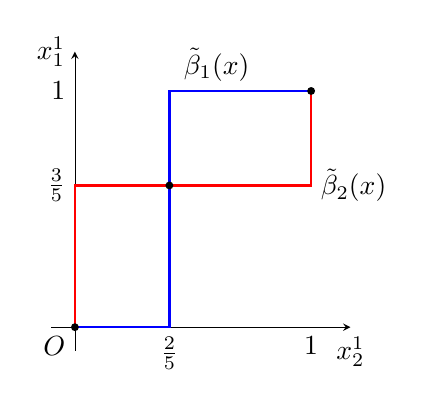
\begin{tikzpicture}
  \coordinate (XS) at (-0.3,0); %x軸最小
  \coordinate[label=below left:{$O$}] (O) at (0, 0); %原点
  \coordinate[label=below:{$x_2^1$}] (XL) at (3.5,0); %x軸最大
  \coordinate[label=below:{$1$}] (X1) at (3, 0); %x_2^1 = 1
  \draw[very thin,->,>=stealth] (XS)--(XL); %x軸
  \coordinate (YS) at (0, -0.3); %y軸最小
  \coordinate[label=left:{$x_1^1$}] (YL) at (0, 3.5); %y軸最大
  \coordinate[label=left:{$1$}] (Y1) at (0, 3); %x_1^1 = 1
  \draw[very thin,->,>=stealth] (YS)--(YL); %y軸
  \coordinate[label=below:{$\frac{2}{5}$}] (alp2) at (1.2, 0); %alpha_2
  \coordinate (alp2_1) at (1.2, 3);
  \coordinate[label=left:{$\frac{3}{5}$}] (alp1) at (0, 1.8); %alpha_1
  \coordinate (alp1_1) at (3, 1.8);
  \coordinate (I) at (3, 3); %(1, 1)
  \coordinate (crs) at (1.2, 1.8);
  \draw[thick, blue] (O)--(alp2)--(alp2_1)--(I);
  \draw[thick, red] (O)--(alp1)--(alp1_1)--(I);
  \coordinate[label=above:{$\tilde{\beta}_1(x)$}] (beta1) at (1.8, 3); % beta_1(x)
  \coordinate[label=right:{$\tilde{\beta}_2(x)$}] (beta2) at (3, 1.8); % beta_2(x)
  \fill (I) circle[radius=0.5mm];
  \fill (crs) circle[radius=0.5mm];
  \fill (O) circle[radius=0.5mm];
\end{tikzpicture}

\end{document}
